%% chapter04_slides.tex
%% Chapter 4: Solving Problems That Have Dual Solution Characteristics
%% Nature Inspired Optimisation for Delivery Problems (2022)
%% Self-contained lecture slides — complete sentences, all symbols explained
\documentclass[aspectratio=169,10pt]{beamer}

\usetheme{Madrid}
\usecolortheme{seahorse}

\usepackage[utf8]{inputenc}
\usepackage[T1]{fontenc}
\usepackage{amsmath,amssymb}
\usepackage{booktabs}
\usepackage{array}
\usepackage{listings}
\usepackage{xcolor}
\usepackage{graphicx}
\usepackage{hyperref}
\usepackage{tikz}
\usepackage{microtype}
\usepackage{multirow}

\graphicspath{{figures/}}

\setbeamertemplate{footline}[frame number]
\setbeamertemplate{navigation symbols}{}

% ── listings style ──────────────────────────────────────────────────────────
\lstset{
  language=Python,
  basicstyle=\ttfamily\scriptsize,
  numbers=left,
  numberstyle=\tiny\color{gray},
  frame=single,
  backgroundcolor=\color{gray!7},
  commentstyle=\color{green!50!black}\itshape,
  keywordstyle=\color{blue!80!black}\bfseries,
  stringstyle=\color{orange!80!black},
  showstringspaces=false,
  breaklines=true,
  xleftmargin=1.5em,
  framexleftmargin=1.5em,
  tabsize=4,
}

% Java style for code from the book
\lstdefinelanguage{JavaBook}{
  language=Java,
  basicstyle=\ttfamily\scriptsize,
  numbers=left,
  numberstyle=\tiny\color{gray},
  frame=single,
  backgroundcolor=\color{gray!7},
  commentstyle=\color{green!50!black}\itshape,
  keywordstyle=\color{blue!80!black}\bfseries,
  stringstyle=\color{orange!80!black},
  showstringspaces=false,
  breaklines=true,
  xleftmargin=1.5em,
  framexleftmargin=1.5em,
  tabsize=4,
}

% ── title page ───────────────────────────────────────────────────────────────
\title[Ch.4 Dual Objectives]{Chapter 4: Solving Problems That Have\\
  Dual Solution Characteristics}
\subtitle{Nature Inspired Optimisation for Delivery Problems (2022)}
\author{}
\date{}

\begin{document}

\begin{frame}
  \titlepage
\end{frame}

% ── outline ──────────────────────────────────────────────────────────────────
\begin{frame}{Chapter Outline}
  \tableofcontents
\end{frame}

\section{4.1 Dealing with Conflicting Objectives}

\begin{frame}[allowframebreaks]{4.1 Why One Objective Is Often Not Enough}

  Real-world delivery problems almost always involve tension between two or more
  goals that pull in opposite directions.  A typical logistics manager cares about
  at least two things simultaneously: \emph{cost} (keeping transport expenditure
  low) and \emph{environmental impact} (reducing fuel consumption and emissions).
  Unfortunately, trying to minimise one of these two objectives usually makes the
  other one worse.

  \begin{block}{The Fundamental Tension}
    A solution that minimises cost typically achieves this by consolidating
    deliveries onto as few vehicles as possible, meaning each vehicle carries a
    heavy load and travels long, winding routes --- which increases emissions and
    environmental impact.  Conversely, minimising environmental impact may call for
    fewer kilometres driven, which can require more vehicles and thus higher
    operational costs.
  \end{block}

  \framebreak

  Before this chapter, the ACE Doughnuts logistics team used a single-objective
  approach: they would pick one criterion --- say, total distance --- as the fitness
  function, and the Evolutionary Algorithm (EA) would return a \emph{single}
  best solution.  However, the logistics manager found this approach frustrating.
  The returned solution did not always match their needs.

  \begin{exampleblock}{A Concrete Illustration}
    Suppose the single-objective EA returns a solution with 5 routes and a
    customer service metric of 5{,}466.  This may be excellent for minimising
    routes, but the customer service level (lower is better in the book's
    formulation) may be far worse than what the manager actually needs.
    Meanwhile, optimising customer service alone may yield a solution with
    32~routes --- far too many vehicles for the available fleet.
  \end{exampleblock}

  \framebreak

  There are three different types of result that can emerge from a bi-objective
  optimisation.  Understanding these three cases is essential before we go further.

  \begin{enumerate}
    \item \textbf{Find a solution that optimises} $c$ \textbf{(cost, say) at the
      expense of} $e$ \textbf{(environment)}.  This is the extreme point where $c$
      is as small as possible, with no regard for $e$.
    \item \textbf{Find a solution that optimises} $e$ \textbf{at the expense of}
      $c$.  This is the opposite extreme.
    \item \textbf{Find a range of trade-off solutions} that balance $c$ and $e$
      in different proportions, allowing a human decision-maker to choose the
      trade-off that suits their current situation.
  \end{enumerate}

  The third option is by far the most useful in practice, and it is the main
  subject of this chapter.  We want to present the decision-maker with a
  \emph{set} of solutions, not just one.

  \framebreak

  \begin{alertblock}{Key Insight}
    The goal of multi-objective optimisation is not to find \emph{the} best
    solution, but to find the best \emph{set} of solutions, each representing a
    different trade-off between the competing objectives.  This empowers the human
    expert to make an informed final decision, taking into account factors that are
    difficult to quantify mathematically.
  \end{alertblock}

  \begin{center}
    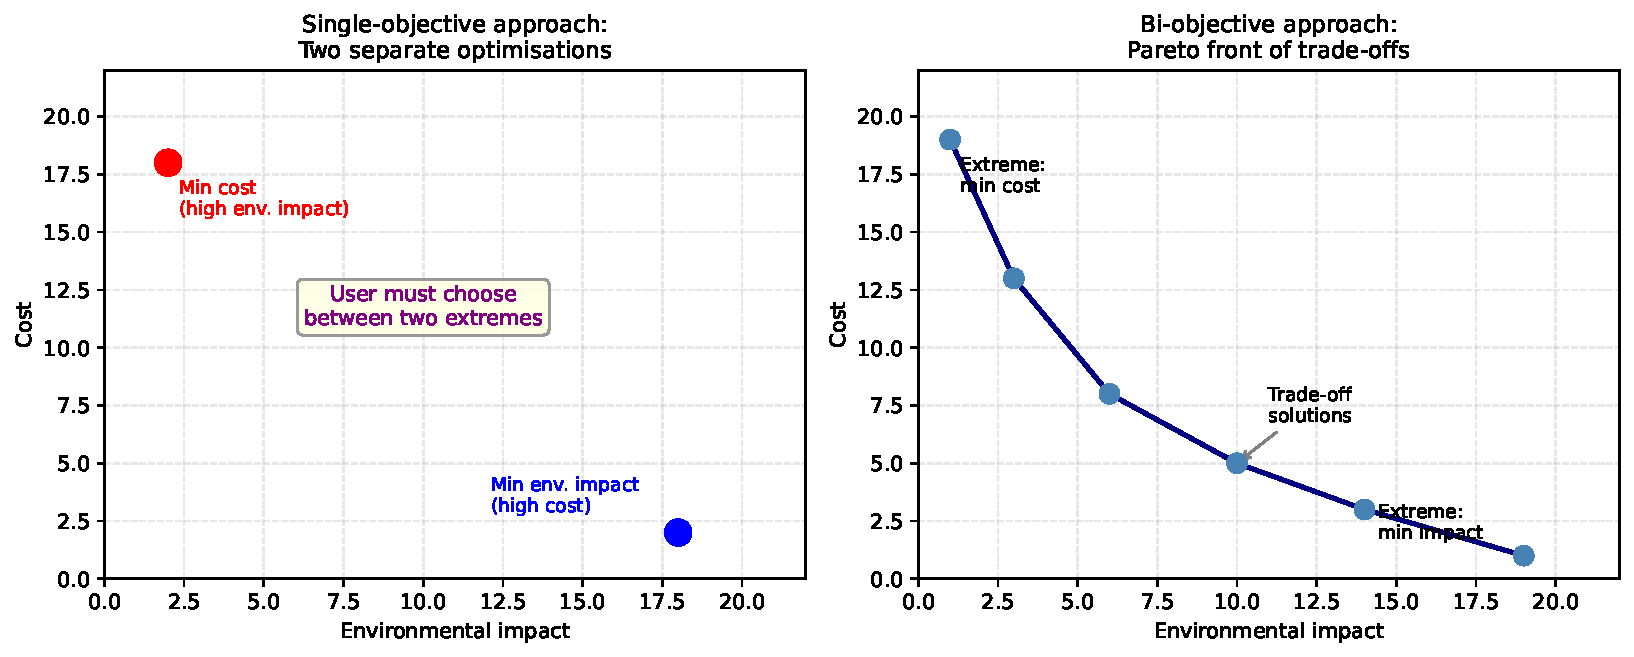
\includegraphics[width=0.80\textwidth]{fig_tradeoff_illustration.pdf}
  \end{center}

  On the left, single-objective optimisation yields only two extreme points --- no
  middle ground is visible.  On the right, bi-objective optimisation yields a full
  curve of trade-off solutions from which the manager can select.

\end{frame}

\section{4.2 Pareto Dominance}

\begin{frame}[allowframebreaks]{4.2 Pareto Dominance --- Formal Definition}

  Named after the Italian economist \textbf{Vilfredo Pareto} (1848--1923), who
  observed that in economics, resource allocations can be improved without
  making anyone worse off until a certain boundary is reached --- the
  ``Pareto optimal'' boundary.  In optimisation, we adopt a similar idea.

  We consider solutions that have two measurable characteristics, which we wish
  to \emph{minimise}.  Let us call these characteristics $c$ and $e$.

  \begin{block}{Definition: Pareto Dominance (minimisation)}
    Solution $x_1$ \textbf{dominates} solution $x_2$ --- written $x_1 \prec x_2$
    --- if and only if:
    \begin{align}
      c(x_1) &\leq c(x_2) \quad \text{(at least as good on } c \text{)} \\
      e(x_1) &\leq e(x_2) \quad \text{(at least as good on } e \text{)} \\
              &\text{and at least one inequality is strict.}
    \end{align}
    \textbf{Symbols:} $c(x_1)$ is the cost of solution $x_1$; $e(x_1)$ is its
    environmental impact.  The symbol ``$\leq$'' means ``less than or equal to''.
    A strict inequality means ``strictly less than''.
  \end{block}

  In plain English: $x_1$ dominates $x_2$ when $x_1$ is \emph{at least as good}
  on every objective, and \emph{strictly better} on at least one.  There is no
  reason to ever choose $x_2$ over $x_1$.

  \framebreak

  \begin{exampleblock}{Worked Numerical Example}
    Consider three solutions with characteristics $(c, e)$:
    \begin{center}
      \begin{tabular}{ccc l}
        \toprule
        Solution & $c$ & $e$ & Verdict \\
        \midrule
        $x_A$ & 5  & 7  & Non-dominated (our reference solution A) \\
        $x_1$ & 12 & 8  & Dominated by $x_A$ (A has $c=5 < 12$ and $e=7 < 8$) \\
        $x_2$ & 9  & 14 & Dominated by $x_A$ (A has $c=5 < 9$ and $e=7 < 14$) \\
        $x_3$ & 14 & 15 & Dominated by $x_A$ (A has $c=5 < 14$ and $e=7 < 15$) \\
        \bottomrule
      \end{tabular}
    \end{center}
    Solution $x_A = (5, 7)$ dominates all three because it is strictly better on
    both $c$ and $e$.  Since no other solution dominates $x_A$ itself, $x_A$ is
    called \textbf{non-dominated}.
  \end{exampleblock}

  \framebreak

  \begin{center}
    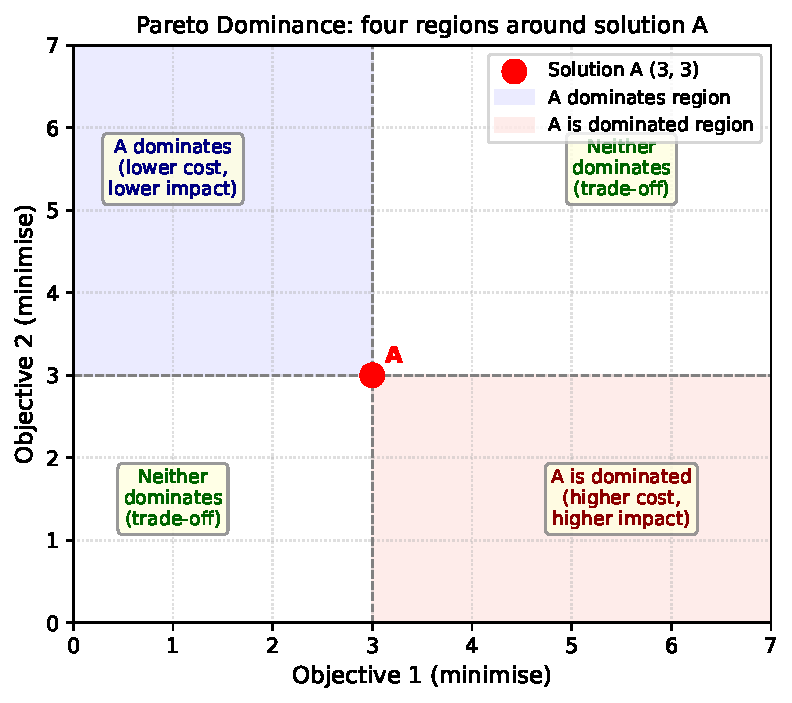
\includegraphics[width=0.55\textwidth]{fig_dominance_concept.pdf}
  \end{center}

  The plot shows the four possible quadrants around any solution $A$.  For
  minimisation:

  \begin{itemize}
    \item Solutions in the \textbf{lower-left} quadrant (smaller $c$ AND smaller
      $e$ than $A$) dominate $A$.
    \item Solutions in the \textbf{upper-right} quadrant (larger $c$ AND larger
      $e$ than $A$) are dominated \emph{by} $A$.
    \item Solutions in the remaining two quadrants are \textbf{incomparable} to
      $A$ --- neither dominates the other.  These represent genuine trade-offs.
  \end{itemize}

  \framebreak

  \begin{center}
    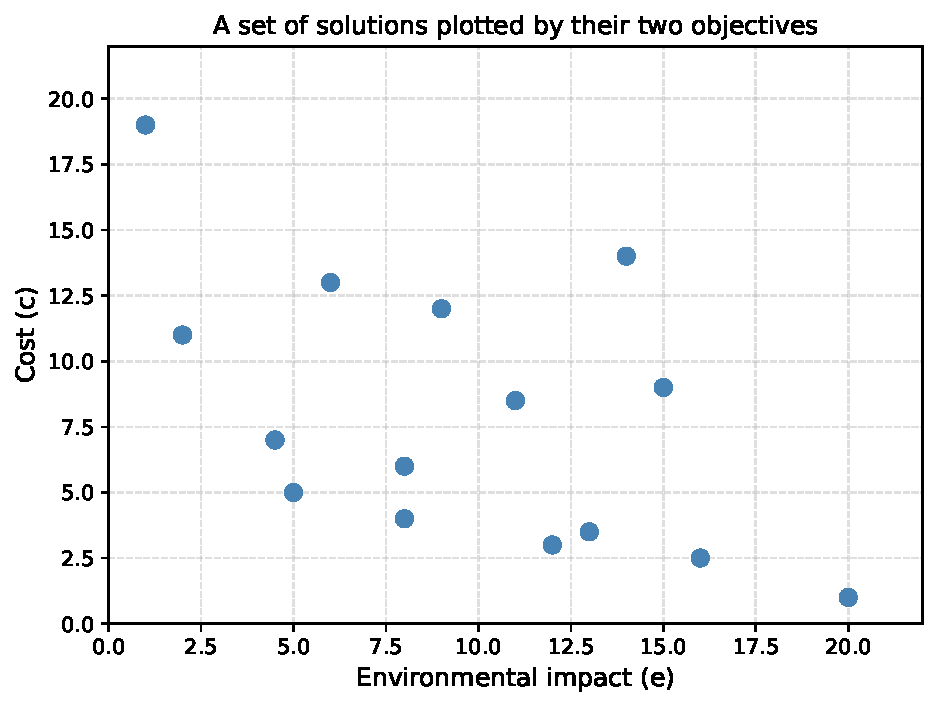
\includegraphics[width=0.80\textwidth]{fig_scatter_solutions.pdf}
  \end{center}

  The scatter plot shows a set of candidate solutions in the objective space (cost
  $c$ on the $y$-axis, environmental impact $e$ on the $x$-axis).  We wish to
  find which of these solutions are dominated and which are not.

  \framebreak

  \begin{center}
    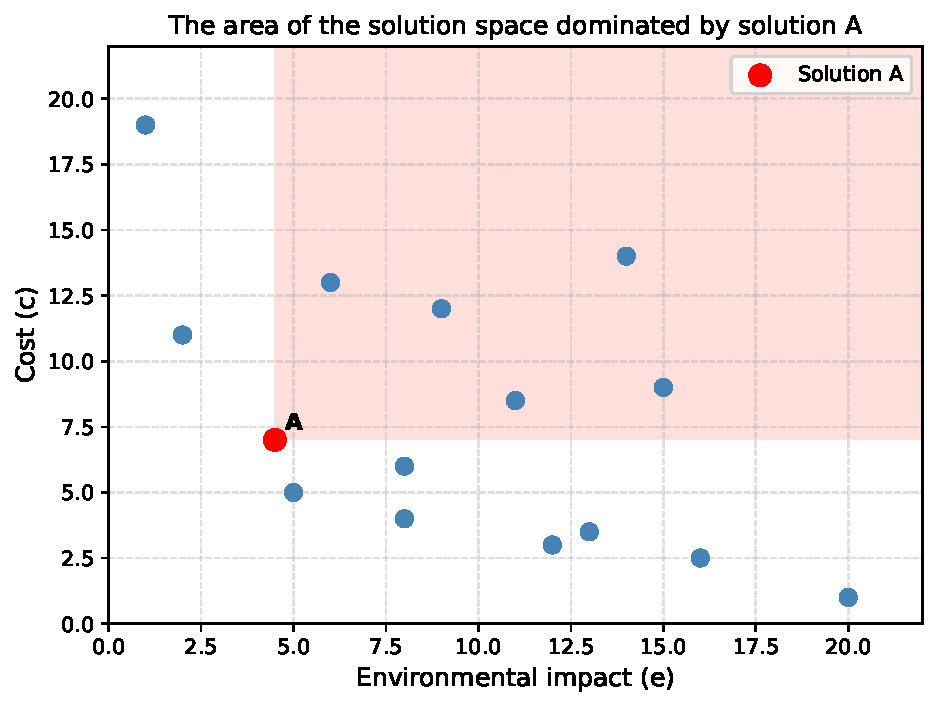
\includegraphics[width=0.80\textwidth]{fig_dominated_region.pdf}
  \end{center}

  The shaded region shows the area of the objective space that is dominated by
  solution $A$ at coordinates $(5, 7)$.  Any solution that falls inside this
  shaded upper-right rectangle is strictly worse than $A$ on both objectives, so
  the user has no reason to choose those solutions.

  \framebreak

  \begin{center}
    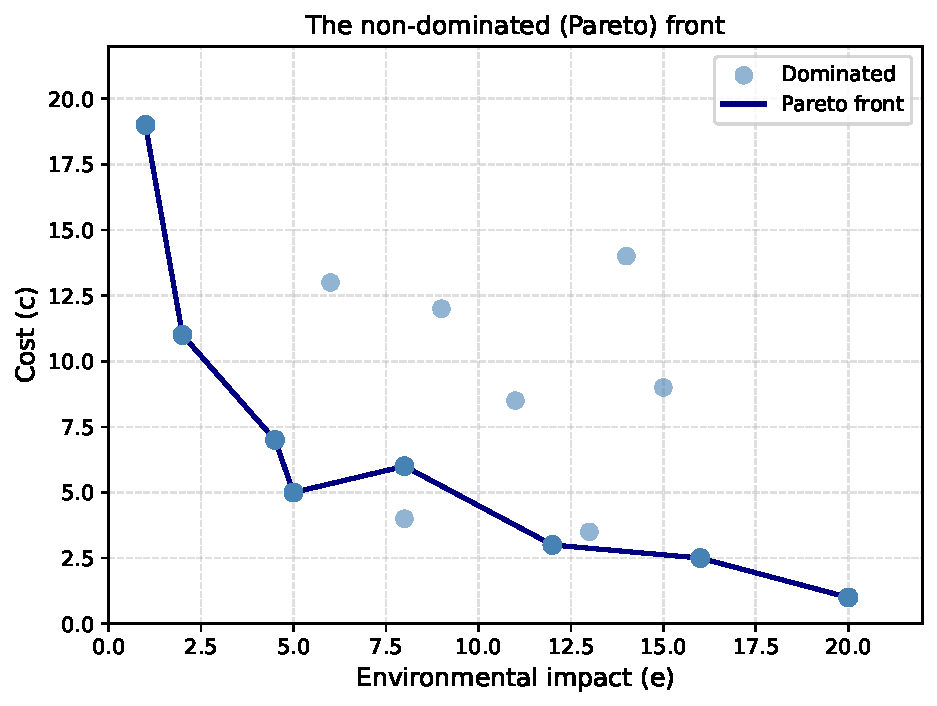
\includegraphics[width=0.80\textwidth]{fig_pareto_front.pdf}
  \end{center}

  After checking all pairs of solutions for dominance, the non-dominated solutions
  form a front --- the \textbf{Pareto front}.  These are the only solutions worth
  presenting to the user.

  \begin{block}{The Non-Dominated Front in Numbers}
    \begin{center}
      \small
      \begin{tabular}{cc l}
        \toprule
        $c$ & $e$ & Role \\
        \midrule
        20 & 1  & Extreme: minimises $c$ \\
        11 & 3  & Trade-off \\
        7  & 5  & Trade-off \\
        5  & 12 & Trade-off \\
        3  & 16 & Trade-off \\
        1  & 20 & Extreme: minimises $e$ \\
        \bottomrule
      \end{tabular}
    \end{center}
  \end{block}

  At the head of this list we have the solution that minimises $c$ (cost) but at
  the expense of high $e$ (environmental impact).  At the tail we have the
  reverse.  The intermediate solutions represent genuine trade-offs where a small
  reduction in $c$ can be bought at a modest increase in $e$.

\end{frame}

\begin{frame}[allowframebreaks]{4.2 Algorithm: Finding the Non-Dominated Front}

  We now need a concrete algorithm that takes a population of solutions and
  extracts only those that are non-dominated.  The logic is straightforward: for
  each solution in the population, check whether any \emph{other} solution
  dominates it.  If none does, it belongs to the non-dominated front.

  \begin{block}{Algorithm 11: FindNonDomFront}
    \begin{enumerate}
      \item Initialise an empty list \texttt{nonDom}.
      \item For each solution \texttt{possible} in the population:
        \begin{enumerate}
          \item Set \texttt{dominated = False}.
          \item For each \emph{other} solution in the population:
            \begin{itemize}
              \item If that other solution dominates \texttt{possible}, set
                \texttt{dominated = True} and stop checking (break).
            \end{itemize}
          \item If \texttt{dominated} is still \texttt{False}, add
            \texttt{possible} to \texttt{nonDom}.
        \end{enumerate}
      \item Return \texttt{nonDom}.
    \end{enumerate}
  \end{block}

  The time complexity of this algorithm is $O(n^2)$ in the number of solutions
  $n$, because in the worst case every solution is checked against every other
  solution.  For large populations this can be expensive, and faster algorithms
  exist (such as NSGA-II's fast non-dominated sort), but Algorithm 11 is easy to
  understand and implement.

  \framebreak

  The Python implementation below translates the algorithm directly.  The helper
  method \texttt{dominates(self, other)} returns \texttt{True} if the current
  solution dominates \texttt{other}, meaning it is at least as good on all
  objectives and strictly better on at least one.

\end{frame}

\begin{frame}[fragile]{Python: Finding the Non-Dominated Front}
\begin{lstlisting}
def dominates(self_vec, other_vec):
    """Return True if self_vec dominates other_vec (minimisation).

    self_vec and other_vec are lists of objective values,
    e.g. [cost, env_impact].

    'dominates' means: no worse on any objective,
    strictly better on at least one.
    """
    at_least_as_good = all(s <= o for s, o in zip(self_vec, other_vec))
    strictly_better  = any(s <  o for s, o in zip(self_vec, other_vec))
    return at_least_as_good and strictly_better


def find_non_dom_front(population):
    """Extract the non-dominated solutions from a population.

    population: list of objects, each with a .get_vector() method
                returning a list of objective values.
    Returns: list of non-dominated solution objects.
    """
    non_dom = []
    for candidate in population:
        dominated = False
        for other in population:
            if other is candidate:
                continue  # do not compare a solution to itself
            if dominates(other.get_vector(), candidate.get_vector()):
                dominated = True
                break      # no need to check further -- already dominated
        if not dominated:
            non_dom.append(candidate)
    return non_dom


# -- Worked example with numerical solutions --------------------------------
class Solution:
    def __init__(self, cost, env):
        self.cost = cost
        self.env  = env
    def get_vector(self):
        return [self.cost, self.env]
    def __repr__(self):
        return f"Solution(c={self.cost}, e={self.env})"

population = [
    Solution(20,  1),   # extreme: min cost
    Solution(11,  3),
    Solution( 7,  5),
    Solution( 5, 12),
    Solution( 3, 16),
    Solution( 1, 20),   # extreme: min env-impact
    Solution(12,  8),   # dominated
    Solution( 9, 14),   # dominated
    Solution(14, 14),   # dominated
]

front = find_non_dom_front(population)
print("Non-dominated front:")
for s in front:
    print(f"  {s}")
\end{lstlisting}
\begin{exampleblock}{Output}
\texttt{Non-dominated front: Solution(c=20,e=1), Solution(c=11,e=3),
Solution(c=7,e=5), Solution(c=5,e=12), Solution(c=3,e=16), Solution(c=1,e=20)}
\end{exampleblock}
\end{frame}

\section{4.3 NSGA-II: An Evolutionary Algorithm for Non-Dominated Fronts}

\begin{frame}[allowframebreaks]{4.3 Adapting the Evolutionary Algorithm for Two Objectives}

  In Chapter 3, the Evolutionary Algorithm (EA) used a single \emph{fitness
  function} --- a number indicating how good a solution was --- to drive
  selection.  Better fitness meant a higher chance of becoming a parent and
  producing offspring.  With two objectives, there is no single number that
  captures ``better''; instead, we have the concept of \emph{dominance}.

  \begin{block}{Core Idea: Selection by Dominance}
    Instead of selecting the solution with the better fitness score, we select the
    solution that \emph{dominates} the other.  If neither dominates the other
    (they are incomparable), we keep one arbitrarily --- both are equally
    acceptable trade-offs.
  \end{block}

  The modified selection mechanism is called \textbf{dominated tournament
  selection} (Algorithm 12 in the book).  It picks two solutions at random from
  the population.  If one dominates the other, the dominating solution is chosen
  as a parent.  If neither dominates, either can be chosen.

  \framebreak

  \begin{block}{Algorithm 12: DominatedTournament}
    \begin{enumerate}
      \item Pick solution $x$ at random from the population.
      \item Pick solution $y$ at random from the population.
      \item If $x$ dominates $y$: return $x$.
      \item Otherwise: return $y$.
    \end{enumerate}
  \end{block}

  Note that step 4 returns $y$ regardless of whether $y$ dominates $x$.  This is
  a simplification: since neither dominates the other in the ``otherwise'' case
  (if $y$ dominated $x$, step 3 would have caught it --- actually the condition is
  asymmetric), both are acceptable choices.

  \begin{alertblock}{Important Distinction: Non-Dominated vs.\ Pareto Optimal}
    The EA returns a \emph{non-dominated} front, but not necessarily the
    \emph{Pareto optimal} front.  The Pareto optimal front is the theoretically
    best set of non-dominated solutions, taking into account the \emph{entire}
    solution space.  Because the CVRP (Capacitated Vehicle Routing Problem) is
    NP-Complete (no polynomial-time exact algorithm is known), we cannot guarantee
    finding the Pareto optimal front in a reasonable time.  The EA finds the best
    non-dominated front it can within the given computational budget.
  \end{alertblock}

  \framebreak

  The full evolutionary loop is modified in two important ways compared to the
  single-objective EA from Chapter 3:

  \begin{enumerate}
    \item \textbf{Batch child creation.} Instead of creating one child per
      iteration, we create a batch of \texttt{CHILDREN} children before updating
      the population.  This amortises the cost of the computationally expensive
      non-dominated front extraction.
    \item \textbf{Population pruning by dominance.} After adding all children to
      the population, we reduce the population to only its non-dominated members
      by calling \texttt{extractNonDom()}.  This is what drives the algorithm
      toward the Pareto front over time.
  \end{enumerate}

  The grand front --- formed by combining the non-dominated fronts from multiple
  independent runs --- is defined as:

  \begin{block}{Grand Front Formula}
    \[
      \text{grandFront} = nd(p_1 \cup p_2 \cup \ldots \cup p_{10})
    \]
    where $nd(s)$ is a function that returns the set of non-dominated members
    of set $s$, and $p_n$ (where the subscript $n$ denotes the run number, from
    1 to 10) is the non-dominated front returned by run $n$ of the EA.
  \end{block}

  The union symbol $\cup$ (pronounced ``union'') means we combine all solutions
  from all runs into one large pool, then extract the non-dominated ones.  The
  grand front is at least as good as any individual run's front, and typically
  better because different runs explore different parts of the objective space.

\end{frame}

\begin{frame}[fragile]{Python: Dominated Tournament and EA Main Loop}
\begin{lstlisting}
import random

def dominated_tournament(population):
    """Select a solution using dominance-based tournament.

    Picks two random solutions; returns the one that dominates
    the other, or an arbitrary one if neither dominates.
    """
    x = random.choice(population)
    y = random.choice(population)
    if dominates(x.get_vector(), y.get_vector()):
        return x
    else:
        return y   # y may dominate x, or neither may dominate


def bi_objective_ea(problem, evals_budget=10000,
                    init_pop_size=100, children=10,
                    xo_rate=0.7):
    """Bi-objective Evolutionary Algorithm returning a non-dominated front.

    problem      : the VRP problem instance
    evals_budget : total number of solution evaluations allowed
    init_pop_size: size of the initial random population
    children     : number of children created per iteration (batch size)
    xo_rate      : probability of crossover vs. mutation-only (0.7 = 70%)
    """
    # Step 1: Create initial random population
    population = [BiObjectiveIndividual(problem)
                  for _ in range(init_pop_size)]
    for ind in population:
        ind.evaluate()
    evals_budget -= init_pop_size   # account for evaluations spent

    while evals_budget > 0:
        new_children = []
        for _ in range(children):
            # Step 2: Select parents using domination tournament
            if random.random() < xo_rate:
                parent1 = dominated_tournament(population)
                parent2 = dominated_tournament(population)
                child   = crossover(parent1, parent2, problem)
            else:
                parent = dominated_tournament(population)
                child  = parent.copy()

            child.mutate()
            child.evaluate()
            evals_budget -= 1
            new_children.append(child)

        # Step 3: Add children and prune to non-dominated front
        population.extend(new_children)
        population = find_non_dom_front(population)

    return population  # the non-dominated front


def build_grand_front(problem, n_runs=10, **kwargs):
    """Combine n_runs independent EA fronts into a grand front."""
    all_solutions = []
    for run in range(n_runs):
        front = bi_objective_ea(problem, **kwargs)
        all_solutions.extend(front)
    return find_non_dom_front(all_solutions)
\end{lstlisting}
\end{frame}

\section{4.4 Case Study: Routes Versus Customer Service}

\begin{frame}[allowframebreaks]{4.4 The ACE Doughnuts Bi-Objective Problem}

  ACE Doughnuts returns as our case study.  Previously, the EA returned a single
  solution.  The logistics manager has identified two characteristics that matter
  most when evaluating a delivery plan:

  \begin{enumerate}
    \item \textbf{Number of routes.}  Fewer routes means fewer vehicles and drivers
      are needed, reducing operational costs.  The manager wants to \emph{minimise}
      this.
    \item \textbf{Customer service metric.}  This measures how well delivery times
      are distributed across customers --- essentially a fairness and service quality
      score.  A lower value (in the book's formulation) means better service because
      customers receive their orders closer to their preferred times.  The manager
      also wants to \emph{minimise} this.
    \end{enumerate}

  These two objectives conflict with each other in a direct and obvious way.
  Reducing the number of routes means each vehicle serves more customers, which
  means longer and less tailored routes, which degrades customer service.
  Improving customer service means allocating each customer to a more specific
  route, which requires more routes overall.

  \framebreak

  \begin{alertblock}{Why Single-Objective Results Are Unsatisfactory}
    Table 4.1 in the book shows that optimising for routes alone can yield a
    customer service metric of 8{,}051.56 for problem A-n32-k5, while optimising
    for customer service alone yields 5{,}466.66 for the same problem.  Neither
    extreme satisfies the manager, who wants a \emph{choice} between these
    extremes.
  \end{alertblock}

  \begin{block}{A Sample of Single-Objective Results (Problem Set A)}
    \small
    \begin{tabular}{l rr | rr}
      \toprule
      Problem & \multicolumn{2}{c|}{Minimise Routes} & \multicolumn{2}{c}{Minimise Cust.\ Svc.} \\
              & Routes & Cust.\ Svc. & Routes & Cust.\ Svc. \\
      \midrule
      A-n32-k5 & 5 & 8051.56 & 5 & 5466.66 \\
      A-n33-k5 & 5 & 5231.27 & 6 & 3428.42 \\
      A-n33-k6 & 6 & 4748.40 & 6 & 2887.23 \\
      A-n34-k5 & 5 & 6351.24 & 6 & 4360.70 \\
      A-n36-k5 & 5 & 8597.31 & 6 & 5498.88 \\
      \bottomrule
    \end{tabular}
  \end{block}

  The table shows that the ``best'' number of routes depends on which objective is
  being optimised, and the two objectives genuinely conflict across all problem
  instances.

\end{frame}

\begin{frame}[allowframebreaks]{4.4 A New Encoding for Bi-Objective VRP}

  To allow the EA to explore the trade-off between routes and customer service,
  the solution representation (encoding) must be modified.  The original
  representation was simply a permutation of customer visits.  The decoder then
  built routes by splitting the permutation at vehicle capacity boundaries.

  The new representation introduces a \textbf{``new route'' flag} on each gene.
  Each gene now encodes \emph{two} pieces of information:
  \begin{enumerate}
    \item The \textbf{customer ID} to be visited.
    \item A \textbf{Boolean flag} (\texttt{True}/\texttt{False}) indicating
      whether this visit should be placed at the start of a \emph{new route},
      regardless of the current route's remaining capacity.
  \end{enumerate}

  \begin{block}{Example Genotype}
    \begin{center}
      \begin{tabular}{|c|c|c|c|c|}
        \hline
        A, False & B, True & C, False & D, True & E, True \\
        \hline
      \end{tabular}
    \end{center}
    With vehicle capacity 5 and demands $A=2, B=3, C=2, D=1, E=2$.
  \end{block}

  \framebreak

  The decoder now processes the genotype gene by gene.  Whenever it encounters a
  gene with the ``new route'' flag set to \texttt{True}, it immediately starts a
  new route --- even if the current route still has remaining capacity.

  \begin{center}
    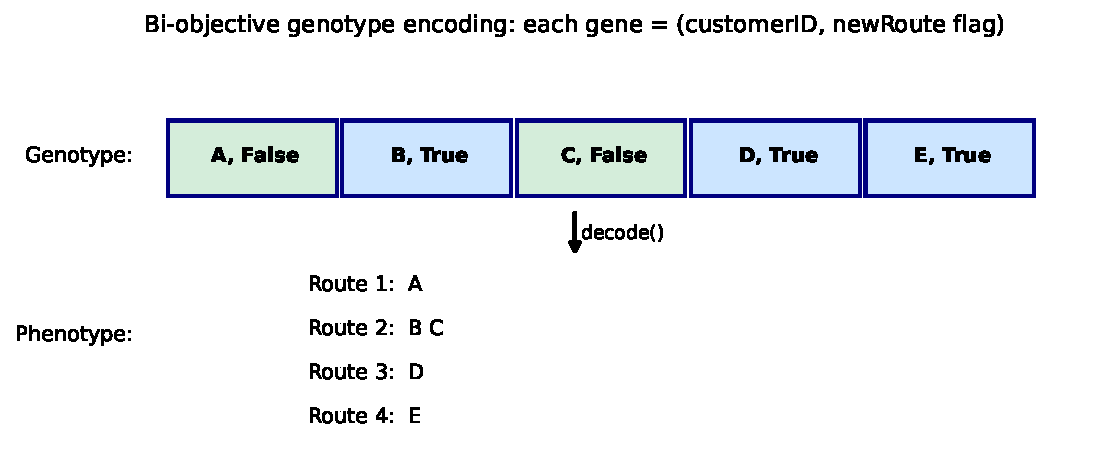
\includegraphics[width=0.78\textwidth]{fig_encoding.pdf}
  \end{center}

  For the example genotype above, the decoder produces four routes:

  \begin{center}
    \small
    \begin{tabular}{cc}
      \toprule
      Route & Customers \\
      \midrule
      1 & A \\
      2 & B C \\
      3 & D \\
      4 & E \\
      \bottomrule
    \end{tabular}
  \end{center}

  Route 1 starts with customer A (no new-route flag yet, first gene).  Route 2
  starts because B has \texttt{newRoute = True}.  Route 3 starts because D has
  \texttt{newRoute = True}.  Route 4 starts because E has \texttt{newRoute = True}.
  Note that without any \texttt{True} flags, the original capacity-based decoder
  behaviour is preserved.

  \framebreak

  \begin{alertblock}{Search Space Explosion}
    The new representation increases the search space dramatically.  Previously,
    with $n$ customers, the search space was $n!$ permutations (the factorial of
    $n$, i.e.\ the number of ways to arrange $n$ items in a sequence).  Now, for
    each of those $n!$ permutations, there are $2^n$ possible binary strings (each
    of $n$ genes can independently be \texttt{True} or \texttt{False}).  The
    combined search space grows to $n! \times 2^n$.
  \end{alertblock}

  \begin{center}
    \small
    \begin{tabular}{r r r}
      \toprule
      $n$ (customers) & $n!$ & $n! \times 2^n$ \\
      \midrule
      1 & 1    & 2 \\
      2 & 2    & 8 \\
      3 & 6    & 48 \\
      4 & 24   & 384 \\
      5 & 120  & 3{,}840 \\
      \bottomrule
    \end{tabular}
  \end{center}

  Even for just 5 customers, the search space is 32 times larger than before.
  This makes exhaustive search impossible for real problem sizes, and reinforces
  why heuristic methods like the EA are necessary.

  \framebreak

  \begin{center}
    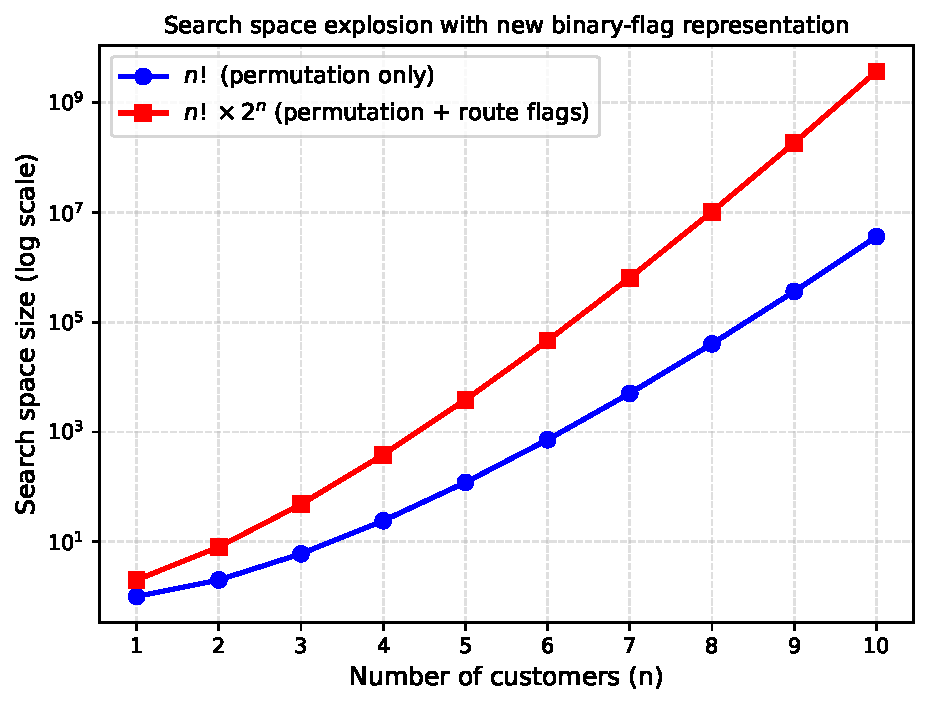
\includegraphics[width=0.72\textwidth]{fig_search_space.pdf}
  \end{center}

  The logarithmic plot (log scale on the $y$-axis means each grid line represents
  a tenfold increase) shows how rapidly the new search space grows compared to the
  original permutation-only space.  For $n = 10$ customers, the bi-objective
  search space has more than a million times more solutions than the original.

  \framebreak

  \begin{block}{Mutation Operator Modification}
    The mutation operator must now handle both the permutation part and the
    Boolean flag part.  With probability 0.5, the mutation selects the classic
    ``swap'' operation (swapping two customers in the permutation).  With the
    remaining probability 0.5, it \emph{flips} the new-route flag of a randomly
    chosen gene: \texttt{True} becomes \texttt{False} and vice versa.
  \end{block}

  Flipping a single new-route flag can change the number of routes by 1, which
  directly affects both objectives simultaneously.  This is the mechanism by which
  the EA navigates the trade-off between fewer routes and better customer service.

\end{frame}

\begin{frame}[fragile]{Java: The Gene Class (Bi-Objective Encoding)}
\begin{lstlisting}[language=JavaBook]
private class Gene {
    /*
     * Represents a single Gene within the bi-objective individual.
     * visit    - the customer visit being made
     * newRoute - true if this visit should start a NEW route
     */
    private boolean newRoute = false;
    private VRPVisit visit   = null;

    public Gene(VRPVisit aVisit) {
        this.visit    = aVisit;
        this.newRoute = false;   // default: no forced new route
    }

    public boolean newRoute() { return this.newRoute; }
    public VRPVisit visit()   { return this.visit; }

    public void setNewRoute(boolean val) { this.newRoute = val; }

    // flipNewRoute() toggles the flag: True->False or False->True
    public void flipNewRoute() {
        this.newRoute = !this.newRoute;
    }
}
\end{lstlisting}
\begin{exampleblock}{Explanation}
  Each Gene object holds two fields.  The \texttt{visit} field (of type
  \texttt{VRPVisit}) stores the customer to be visited.  The \texttt{newRoute}
  flag (a boolean: either \texttt{true} or \texttt{false}) controls whether the
  decoder starts a fresh route at this customer.  The \texttt{flipNewRoute()}
  method is called by the mutation operator to toggle this flag.
\end{exampleblock}
\end{frame}

\begin{frame}[fragile]{Java: The Modified Decode Method}
\begin{lstlisting}[language=JavaBook]
private void decode() {
    if (phenotype == null) {
        phenotype = new ArrayList<ArrayList<VRPVisit>>();
        ArrayList<VRPVisit> newRoute = new ArrayList<VRPVisit>();

        for (Gene g : genotype) {
            VRPVisit v = g.visit();

            if (g.newRoute()) {
                // Gene says "start a new route here" --
                // force a route break regardless of remaining capacity
                phenotype.add(newRoute);
                newRoute = new ArrayList<VRPVisit>();
            }

            if (v.getDemand() + routeDemand(newRoute)
                    > problem.getCapacity()) {
                // Capacity exceeded -- must start a new route anyway
                phenotype.add(newRoute);
                newRoute = new ArrayList<VRPVisit>();
            }

            newRoute.add(v);
        }
        phenotype.add(newRoute);   // add the final route
    }
}
\end{lstlisting}
\begin{alertblock}{Two Route-Break Conditions}
  A new route is started in two cases: (1) the gene explicitly requests it via
  the \texttt{newRoute} flag (lines 11--13), or (2) the next customer's demand
  would exceed the vehicle's capacity (lines 15--19).  The second condition is
  the same as in the original single-objective decoder.  The first is new.
\end{alertblock}
\end{frame}

\begin{frame}[fragile]{Java: The NonDominatedPop Container and EA Loop}
\begin{lstlisting}[language=JavaBook]
// NonDominatedPop: a population manager that maintains only
// non-dominated solutions
public NonDominatedPop extractNonDom() {
    NonDominatedPop result = new NonDominatedPop();
    for (Domination current : this) {          // for each solution
        boolean dominated = false;
        for (Domination member : this) {       // compare to every other
            if (member.dominates(current)) {   // if 'member' beats 'current'
                dominated = true;
                break;
            }
        }
        if (!dominated)
            result.add(current);               // only non-dominated survive
    }
    return result;
}

// The main EA solve() loop
public void solve() {
    population = new NonDominatedPop(INIT_POP_SIZE, super.theProblem);
    evalsBudget -= INIT_POP_SIZE;

    while (evalsBudget > 0) {
        for (int count = 0; count < CHILDREN; count++) {
            BiObjectiveIndividual child;
            if (rnd.getRnd().nextDouble() < XO_RATE) {
                child = new BiObjectiveIndividual(super.theProblem,
                    (BiObjectiveIndividual) population.getDominator(),
                    (BiObjectiveIndividual) population.getDominator());
            } else {
                child = ((BiObjectiveIndividual)
                    population.getDominator()).copy();
            }
            child.mutate();   child.evaluate();   evalsBudget--;
            population.add(child);
        }
        population = population.extractNonDom(); // prune to front
    }
}
\end{lstlisting}
\end{frame}

\begin{frame}[allowframebreaks]{4.4 Results of the Bi-Objective EA}

  Tables 4.2, 4.3, and 4.4 in the book report the results of the bi-objective EA
  across three sets of CVRP benchmark instances.  For each problem instance, the
  table reports:

  \begin{itemize}
    \item The \textbf{minimum and maximum number of routes} found in the
      non-dominated front (i.e.\ the extreme points on the ``routes'' dimension).
    \item The \textbf{minimum and maximum customer service metric} in the front.
    \item The \textbf{front size}: how many non-dominated solutions are in the
      grand front.
  \end{itemize}

  \begin{block}{Selected Results for Problem Set A}
    \small
    \begin{tabular}{l rrrr r}
      \toprule
      Problem & Min Routes & Max Routes & Min Cust.Svc. & Max Cust.Svc. & Front Size \\
      \midrule
      A-n32-k5 & 5 & 31 & 1870.38 & 6096.56 & 27 \\
      A-n33-k5 & 5 & 33 & 1272.05 & 4264.70 & 29 \\
      A-n39-k5 & 5 & 38 & 1806.09 & 6017.81 & 28 \\
      A-n44-k7 & 6 & 44 & 2019.97 & 7003.61 & 41 \\
      A-n80-k10 & 9 & 80 & 5576.9 & 23670.4 & 63 \\
      \bottomrule
    \end{tabular}
  \end{block}

  The grand front for problem A-n32-k5 contains 27 non-dominated solutions, each
  offering a different trade-off between 5 routes (fewest vehicles but worst
  service) and 31 routes (most vehicles but best service, with customer service
  metric as low as 1{,}870).

  \framebreak

  A visualisation of the non-dominated fronts across multiple runs, and the
  resulting grand front, illustrates how the EA explores the trade-off space.

  \begin{center}
    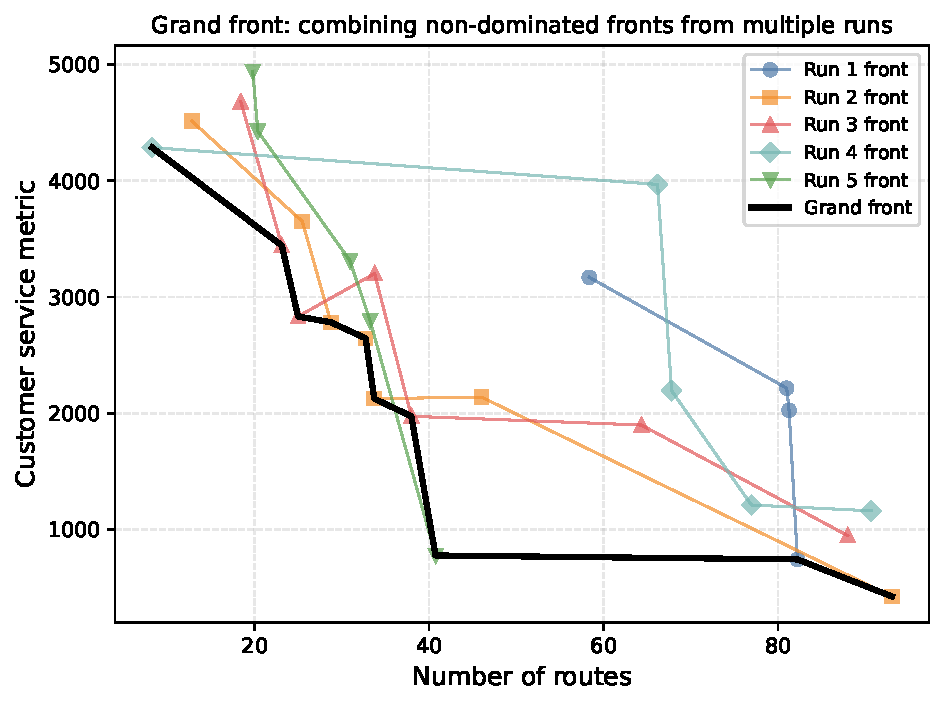
\includegraphics[width=0.72\textwidth]{fig_grand_front.pdf}
  \end{center}

  Each coloured series represents the non-dominated front from a single EA run.
  The black line is the grand front formed by combining all runs.  Notice that the
  grand front lies below and to the left of every individual run's front ---
  meaning it is strictly better than any single run in at least some region.

  \framebreak

  Figure 4.4 in the book shows the initial and final non-dominated fronts for the
  P-n101-k4 problem instance (101 customers, 4 required vehicles).  The initial
  population front is broad and has high customer service values.  After running
  the EA, the final front is substantially improved across the entire range of
  route counts.

  \begin{center}
    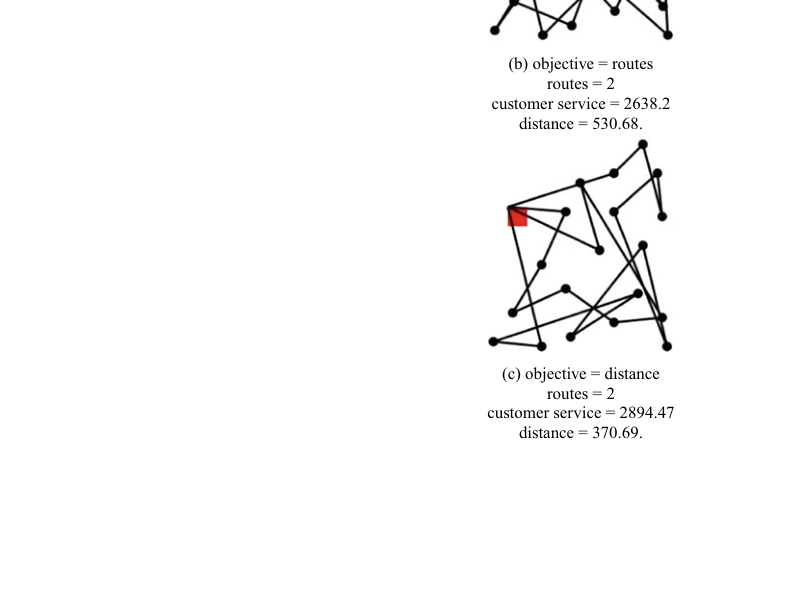
\includegraphics[width=0.72\textwidth]{fig_initial_final_front.png}
  \end{center}

  The extreme solutions on the final front are: (4 routes, customer service
  31{,}644.8) at the routes-minimising end, and (101 routes, customer service
  2{,}494.71) at the customer-service-maximising end.  The book reports that the
  grand front (combining 10 EA runs) is approximately 2.2\% better in Hypervolume
  than the average individual run.

\end{frame}

\section{4.5 Results Summary}

\begin{frame}[allowframebreaks]{4.5 Discussion of Results Across Problem Sets}

  The bi-objective EA was tested on three sets of CVRP benchmark instances (sets
  A, B, and P), covering problems ranging from 16 customers (P-n16-k8) to
  101 customers (P-n101-k4).  The key observations from the results are:

  \begin{enumerate}
    \item \textbf{The lower bound on routes is usually equal to the minimum
      found by single-objective route minimisation.}  This is expected: the
      extreme point of the Pareto front on the routes dimension corresponds to
      the best solution found by the single-objective EA.

    \item \textbf{The upper bound on routes is approximately one route per
      customer} (when all new-route flags are set to \texttt{True}).  This gives
      each customer their own dedicated vehicle for maximum service quality.

    \item \textbf{Customer service improves monotonically as the number of routes
      increases.}  More routes means shorter, more targeted delivery tours, which
      improves the customer service metric.

    \item \textbf{The grand front adds value over individual runs.}  For the
      B-n78-k10 instance, the grand front achieves a Hypervolume 2.2\% above
      the average of the 10 individual run fronts, and 1.9\% above the best
      individual run.
  \end{enumerate}

  \framebreak

  \begin{block}{Grand Front Table for A-n64-k9 (Selected Entries)}
    \small
    \begin{tabular}{rr | rr | rr}
      \toprule
      Routes & Cust.Svc. & Routes & Cust.Svc. & Routes & Cust.Svc. \\
      \midrule
      9  & 14691.63 & 29 & 6429.22 & 52 & 4360.72 \\
      10 & 13448.21 & 30 & 6101.75 & 53 & 4152.55 \\
      11 & 13036.44 & 32 & 5927.05 & 56 & 4096.42 \\
      12 & 11934.61 & 33 & 5728.70 & 57 & 4038.34 \\
      15 & 10960.03 & 36 & 5474.53 & 60 & 3902.84 \\
      20 & 8633.49  & 40 & 5071.66 & 64 & 3816.04 \\
      \bottomrule
    \end{tabular}
  \end{block}

  This table provides the logistics manager with a concrete menu of choices.
  If the manager has a fleet of 20 vehicles, they can see exactly what customer
  service level (8{,}633.49) is achievable.  If they can secure two additional
  vehicles (22 routes), the customer service improves to around 8{,}259.

  \begin{alertblock}{Practical Value}
    The grand front enables scenario analysis.  The planner can ask: ``What is
    the benefit of increasing our fleet from 20 to 25 vehicles?''  The answer is
    read directly from the table: customer service improves from 8{,}633 to
    approximately 7{,}835 --- a 9.3\% improvement for a 25\% fleet increase.
    This kind of cost-benefit analysis is impossible with a single-objective
    approach.
  \end{alertblock}

\end{frame}

\section{4.6 The Hypervolume Indicator}

\begin{frame}[allowframebreaks]{4.6 Comparing Two Non-Dominated Fronts}

  Once we have non-dominated fronts, a natural question arises: how do we compare
  the quality of two different fronts?  For example, if we run two different
  algorithms and each produces a Pareto front, which algorithm produced the better
  front?

  Directly comparing point by point is difficult because the two fronts may have
  different numbers of points at different positions.  We need a single scalar
  (one number) that summarises the quality of an entire front.

  \begin{block}{The Hypervolume Indicator (Definition)}
    The \textbf{Hypervolume Indicator} (also called the S-metric or HV) measures
    the $n$-dimensional volume (in 2D: the area; in 3D: the volume) of the
    \emph{objective space} that is dominated by the non-dominated front and
    bounded by a reference point called the \textbf{nadir point}.

    Formally, for a front $F$ and nadir point $\mathbf{z}_{\text{nadir}}$:
    \[
      \text{HV}(F, \mathbf{z}_{\text{nadir}})
        = \lambda\!\left(
            \bigcup_{x \in F}
            \bigl\{ \mathbf{a} : x \prec \mathbf{a} \prec \mathbf{z}_{\text{nadir}} \bigr\}
          \right)
    \]
    where $\lambda(\cdot)$ denotes the $n$-dimensional Lebesgue measure (i.e.\
    area in 2D, volume in 3D), $x \prec \mathbf{a}$ means $x$ dominates point
    $\mathbf{a}$, and $\mathbf{z}_{\text{nadir}}$ is the nadir point.
  \end{block}

  \framebreak

  \begin{block}{Symbol Guide for the Hypervolume Formula}
    \begin{itemize}
      \item $F$ --- the set of non-dominated solutions (the front).
      \item $\mathbf{z}_{\text{nadir}}$ (nadir point) --- a reference point
        whose coordinates are the \emph{worst} objective values observed across
        all solutions being compared.  In 2D, if the worst cost is 5 and the
        worst environmental impact is 6, then $\mathbf{z}_{\text{nadir}} = (5, 6)$.
      \item $\lambda(\cdot)$ --- the Lebesgue measure, meaning area in 2D or
        volume in 3D.  It is the standard measure of ``size'' of a region.
      \item $\bigcup$ (big union, ``union of all sets'') --- the union over
        all solutions $x$ in the front $F$.
      \item $x \prec \mathbf{a}$ --- solution $x$ dominates point $\mathbf{a}$,
        meaning all coordinates of $x$ are less than or equal to the
        corresponding coordinates of $\mathbf{a}$.
    \end{itemize}
  \end{block}

  \begin{alertblock}{How to Read the Hypervolume Formula}
    The formula builds a region by taking every point in the objective space that
    is dominated by at least one solution in $F$ \emph{and} also dominated by
    the nadir point.  The hypervolume is the total area (or volume) of this
    region.  A larger hypervolume means the front extends further into the
    objective space --- it contains solutions that are better across a wider
    range of trade-offs.  Think of it as: the more area your front ``covers'',
    the better your algorithm is performing.
  \end{alertblock}

  \framebreak

  \begin{center}
    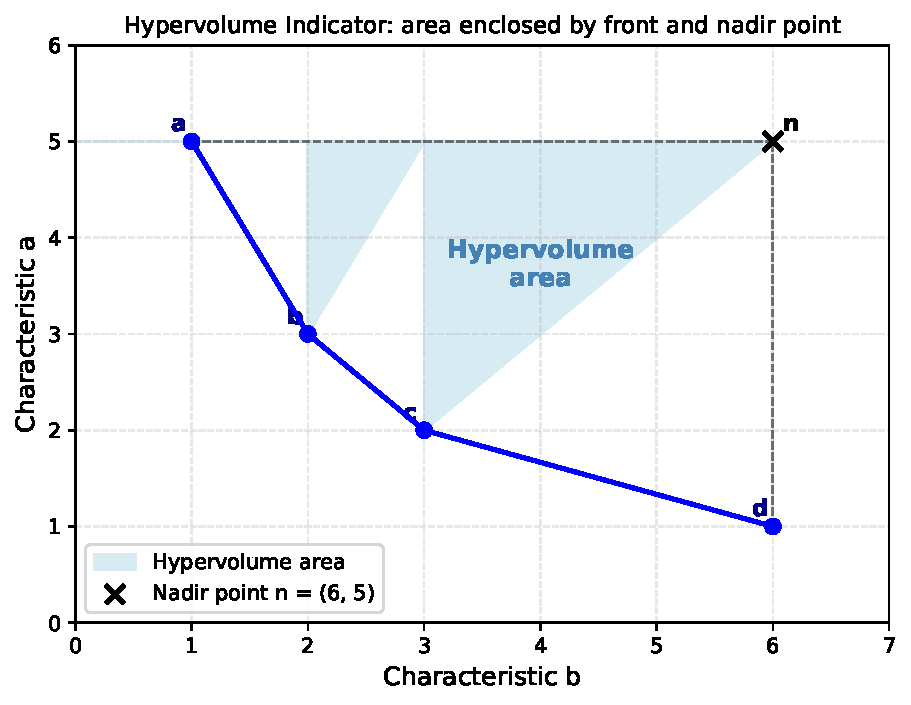
\includegraphics[width=0.78\textwidth]{fig_hypervolume.pdf}
  \end{center}

  The shaded blue region is the hypervolume area for a 2D example.  The front
  consists of four points: $a=(1,5)$, $b=(2,3)$, $c=(3,2)$, $d=(6,1)$.  The
  nadir point is $n=(6,5)$, representing the worst values on both objectives.
  The hypervolume is the area of the blue region.

  \framebreak

  \begin{center}
    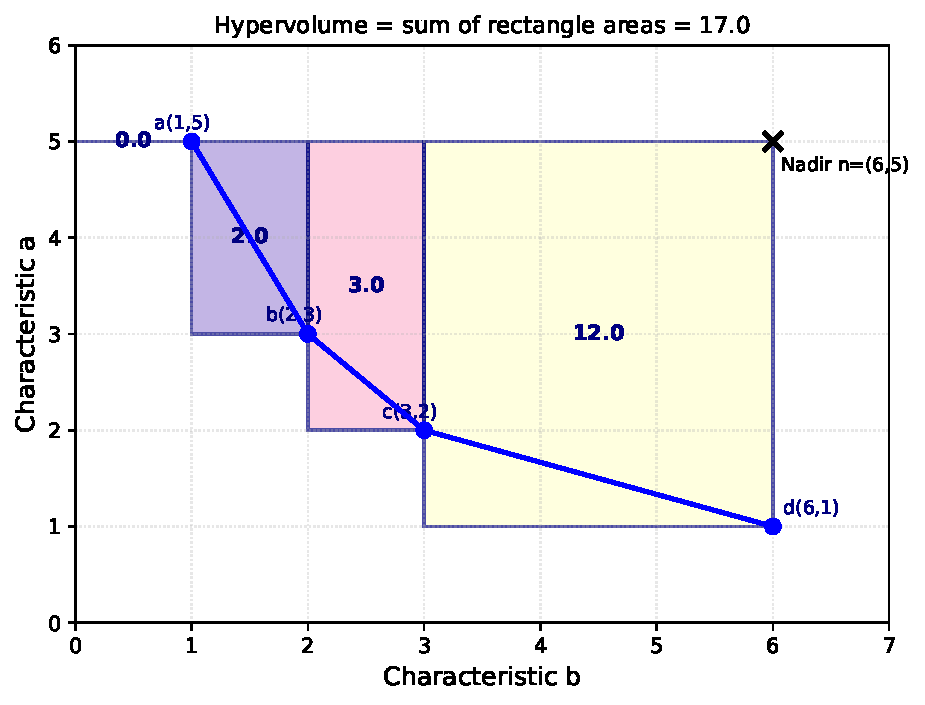
\includegraphics[width=0.78\textwidth]{fig_hypervolume_rectangles.pdf}
  \end{center}

  The hypervolume can be computed exactly in 2D by decomposing the dominated
  region into non-overlapping rectangles.  Each rectangle extends from a front
  point to the nadir line.  The numbers inside the rectangles show the area of
  each strip.

  \framebreak

  \begin{exampleblock}{Worked Numerical Calculation: Hypervolume in 2D}
    Front: $a=(1,5)$, $b=(2,3)$, $c=(3,2)$, $d=(6,1)$.
    Nadir point: $n=(6,5)$.

    We decompose the dominated region into vertical strips (sorted by increasing
    first coordinate):

    \medskip
    \begin{center}
      \small
      \begin{tabular}{ccccc r}
        \toprule
        Strip & $x$-interval & Width & Front $y$ value & Height = Nadir$_y$ $-$ Front$_y$ & Area \\
        \midrule
        1 & $[0, 1)$ & 1 & $y_a = 5$ & $5 - 5 = 0$ & $0.0$ \\
        2 & $[1, 2)$ & 1 & $y_a = 5$ & $5 - 5 = 0$ & $0.0$ \\
        --- & --- & --- & --- & Using staircase approach: & --- \\
        \bottomrule
      \end{tabular}
    \end{center}

    \medskip
    With staircase decomposition from $x=0$ to each front point:

    \begin{itemize}
      \item Rectangle under $a=(1,5)$: width $= 1-0 = 1$,
            height $= 5 - 5 = 0$ $\Rightarrow$ area $= 0$.
      \item Rectangle under $b=(2,3)$: width $= 2-1 = 1$,
            height $= 5 - 3 = 2$ $\Rightarrow$ area $= 2$.
      \item Rectangle under $c=(3,2)$: width $= 3-2 = 1$,
            height $= 5 - 2 = 3$ $\Rightarrow$ area $= 3$.
      \item Rectangle under $d=(6,1)$: width $= 6-3 = 3$,
            height $= 5 - 1 = 4$ $\Rightarrow$ area $= 12$.
    \end{itemize}

    Total Hypervolume $= 0 + 2 + 3 + 12 = \mathbf{17}$.
  \end{exampleblock}

  \framebreak

  \begin{block}{The Nadir Point}
    The nadir point is critical: it acts as the reference point for the
    hypervolume calculation.  Changing the nadir point changes the hypervolume
    value.  When comparing two algorithms, it is \emph{essential} to use the
    same nadir point for both.  Typically, the nadir point is set to the worst
    objective values observed across all solutions from both algorithms being
    compared.
  \end{block}

  In the ACE Doughnuts case study, the book uses the Hypervolume implementation
  released by Fonseca et al.\ (2010), which handles the general multi-dimensional
  case efficiently.

  The key rule is: \textbf{a larger hypervolume is better}.  If algorithm A
  produces a front with hypervolume 599{,}124.83 and algorithm B produces a front
  with hypervolume 586{,}714.55, algorithm A is considered to have found a
  better-quality set of trade-off solutions.

  \framebreak

  \begin{block}{Hypervolume Results for B-n78-k10 (Individual Runs and Grand Front)}
    \begin{center}
      \small
      \begin{tabular}{lr}
        \toprule
        Run / Summary & Hypervolume \\
        \midrule
        Run 1  & 584{,}296.21 \\
        Run 2  & 585{,}481.54 \\
        Run 3  & 588{,}100.99 \\
        Run 4  & 585{,}150.21 \\
        Run 5  & 586{,}476.93 \\
        Run 6  & 586{,}733.97 \\
        Run 7  & 586{,}855.57 \\
        Run 8  & 587{,}436.32 \\
        Run 9  & 588{,}290.44 \\
        Run 10 & 588{,}323.30 \\
        \midrule
        Average         & 586{,}714.55 \\
        Best single run & 588{,}323.30 \\
        \textbf{Grand Front} & \textbf{599{,}124.83} \\
        \bottomrule
      \end{tabular}
    \end{center}
  \end{block}

  The grand front (combining all 10 runs' solutions and extracting the
  non-dominated subset) achieves a hypervolume 2.2\% above the average and 1.8\%
  above the best single run.  This demonstrates the value of aggregating multiple
  runs: the grand front explores regions of the objective space that no single
  run covers fully.

\end{frame}

\begin{frame}[fragile]{Python: Computing the Hypervolume in 2D}
\begin{lstlisting}
def hypervolume_2d(front, nadir):
    """Compute the exact hypervolume for a 2D non-dominated front.

    front : list of (obj1, obj2) tuples, sorted by obj1 ascending.
            Both objectives are to be minimised.
    nadir : (nadir_obj1, nadir_obj2) reference point -- the worst
            values on each objective, used as the upper-right corner.

    Returns the hypervolume (area) as a float.
    """
    # Sort front by first objective ascending (left to right)
    front = sorted(front, key=lambda p: p[0])

    total_area = 0.0
    prev_x = 0.0   # start from x = 0 (or the leftmost bound)

    for (x, y) in front:
        # Width of the current vertical strip
        width  = x - prev_x
        # Height: from nadir_y down to the front's y value
        height = nadir[1] - y

        if height > 0:  # only count if the strip has positive height
            total_area += width * height

        prev_x = x  # advance the left boundary to the current point

    return total_area


# -- Worked example matching the book's Fig 4.5 --------------------------
front = [(1, 5), (2, 3), (3, 2), (6, 1)]   # points a, b, c, d
nadir = (6, 5)                               # nadir point n

hv = hypervolume_2d(front, nadir)
print(f"Hypervolume = {hv:.2f}")
# Expected: 0 + 2 + 3 + 12 = 17.00

# -- Comparing two fronts --------------------------------------------------
front_A = [(1, 5), (2, 3), (3, 2), (6, 1)]
front_B = [(1, 4), (3, 3), (4, 2), (6, 1)]   # slightly different

# Use the same nadir point for fair comparison!
shared_nadir = (6, 5)

hv_A = hypervolume_2d(front_A, shared_nadir)
hv_B = hypervolume_2d(front_B, shared_nadir)

print(f"HV(front A) = {hv_A:.2f}")
print(f"HV(front B) = {hv_B:.2f}")
print(f"Better front: {'A' if hv_A > hv_B else 'B'}")
\end{lstlisting}
\end{frame}

\section{4.7 Conclusions}

\begin{frame}[allowframebreaks]{4.7 Conclusions and Key Takeaways}

  This chapter has introduced the fundamental ideas of multi-objective
  optimisation as applied to vehicle routing problems.  The key concepts are:

  \begin{enumerate}
    \item \textbf{Conflicting objectives are the norm, not the exception.}
      Real delivery planning almost always involves at least two goals that
      trade off against each other.  Trying to solve this with a single
      objective either ignores one concern entirely or requires the user to
      pre-assign weights that are difficult to determine.

    \item \textbf{Pareto dominance provides a natural way to compare solutions
      without needing weights.}  Solution $x_1$ dominates $x_2$ if it is at
      least as good on every objective and strictly better on at least one.
      Non-dominated solutions cannot be improved on any objective without
      degrading another.

    \item \textbf{The Evolutionary Algorithm adapts naturally to multi-objective
      optimisation} by replacing fitness-based selection with dominance-based
      selection.  The rest of the EA infrastructure (crossover, mutation,
      encoding) requires only modest modifications.

    \item \textbf{The Hypervolume Indicator provides a single-number quality
      measure for Pareto fronts}, enabling fair comparison between algorithms
      or between runs of the same algorithm.  A higher hypervolume means a
      better-quality front.

    \item \textbf{The Grand Front, formed by combining multiple EA runs,
      consistently outperforms any single run} as measured by Hypervolume.
      This is because different runs explore different parts of the objective
      space, and their union covers more ground.
  \end{enumerate}

  \framebreak

  \begin{alertblock}{The Broader Philosophical Point}
    The approach in this chapter represents a shift in thinking: instead of
    asking ``what is the best solution?'', we ask ``what is the best
    \emph{set} of solutions?''.  The optimisation algorithm's job is not to
    make the final decision for the logistics manager, but to filter the
    enormous solution space down to a small, high-quality set of trade-offs
    that a human expert can evaluate.
  \end{alertblock}

  This perspective --- multi-objective optimisation as \emph{decision support}
  rather than \emph{decision making} --- is increasingly important as logistics
  problems grow in scale and complexity.

  \framebreak

  \begin{block}{Limitations and Future Directions}
    \begin{itemize}
      \item The bi-objective representation increases the search space by a
        factor of $2^n$ compared to the single-objective representation.
        For large $n$, this can slow convergence.
      \item The distance objective was deliberately excluded in this chapter.
        In the next chapter, we will see how to extend these ideas to
        \emph{three or more} objectives simultaneously.
      \item The non-dominated front found by the EA is not guaranteed to be
        the true Pareto optimal front; it is merely the best approximation
        the algorithm can find within the given evaluation budget.
      \item Different users may have different preferences over the trade-off
        space.  Techniques such as preference articulation, reference point
        methods, and interactive multi-objective optimisation can help guide
        the search toward regions of the front that a particular user cares
        about most.
    \end{itemize}
  \end{block}

  \framebreak

  \begin{block}{Chapter Summary: Concept Map}
    \begin{center}
      \small
      \begin{tabular}{p{3.5cm} p{4.5cm} p{4.5cm}}
        \toprule
        \textbf{Concept} & \textbf{What it is} & \textbf{Why it matters} \\
        \midrule
        Conflicting objectives &
          Two goals that cannot be simultaneously minimised &
          Motivates multi-objective approach \\
        Pareto dominance &
          $x_1 \prec x_2$ if better or equal on all objectives, strictly better on one &
          Defines ``better'' without weights \\
        Non-dominated front &
          Set of solutions no one dominates &
          The useful output for decision-makers \\
        Domination tournament &
          Selection via Pareto dominance &
          Drives EA toward non-dominated solutions \\
        Bi-objective encoding &
          Customer + newRoute flag per gene &
          Allows EA to explore routes vs.\ service trade-off \\
        Grand front &
          Union of fronts from multiple EA runs &
          Better coverage of the Pareto front \\
        Hypervolume &
          Area dominated by the front &
          Single-number quality score for a front \\
        \bottomrule
      \end{tabular}
    \end{center}
  \end{block}

\end{frame}

% ── References ───────────────────────────────────────────────────────────────
\begin{frame}{References}
  \begin{itemize}
    \item Guerreiro, A.P., Fonseca, C.M., Paquete, L.\ (2020).
      \textit{The Hypervolume Indicator: Problems and Algorithms}.
      arXiv:2005.00515.

    \item Fonseca, C.M., Lopez-Ibanez, M., Paquete, L., Guerreiro, A.P.\
      (2010). Computation of the Hypervolume Indicator.
      \url{http://lopez-ibanez.eu/hypervolume}.

    \item Augerat, P.\ (1995). \textit{Approche poly\`edrale du probl\`eme
      de tourn\'ees de v\'ehicules (Polyhedral approach of the vehicle
      routing problem)}. Ph.D.\ Thesis, Grenoble Institute of Technology.

    \item Vilfredo Pareto (2021). Encyclop\ae dia Britannica.
      \url{https://www.britannica.com/biography/Vilfredo-Pareto}.

    \item Deb, K., Pratap, A., Agarwal, S., Meyarivan, T.\ (2002).
      A fast and elitist multiobjective genetic algorithm: NSGA-II.
      \textit{IEEE Transactions on Evolutionary Computation}, 6(2), 182--197.
  \end{itemize}
\end{frame}

\end{document}
